\begin{exercises} 
	\item Let $g$ be the function pictured below at left, and let $F$ be defined by $F(x) = \int_{2}^x g(t) \, dt.$ Assume that the shaded areas have values $A_1 = 4.3$, $A_2 = 12.7$, $A_3 = 0.4$, and $A_4 = 1.8$.  Assume further that the portion of $A_2$ that lies between $x = 0.5$ and $x = 2$ is $5.4$.  
  
  Sketch a carefully labeled graph of $F$ on the axes provided, and include a written analysis of how you know where $F$ is zero, increasing, decreasing, CCU, and CCD. 
  
  \begin{figure}[h]
  \begin{center}
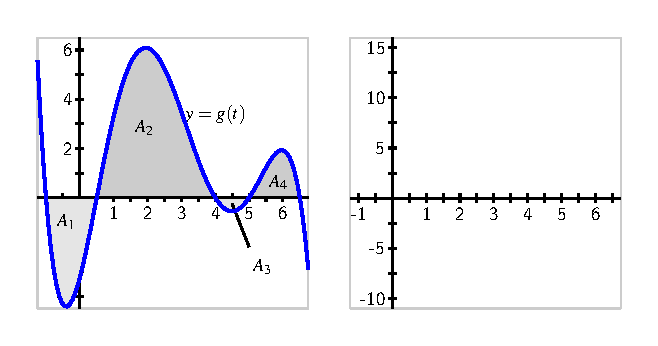
\includegraphics{figures/5_2_Ez1.eps}
\end{center}
\caption{At left, the graph of $g$.  At right, axes for plotting $F$.} \label{F:5.2.Ez1}
  \end{figure}
	
	\item The tide removes sand from the beach at a small ocean park at a rate modeled by the function $$R(t) = 2 + 5\sin \left( \frac{4\pi t}{25} \right)$$
A pumping station adds sand to the beach at rate modeled by the function
$$S(t) = \frac{15t}{1+3t}$$
Both $R(t)$ and $S(t)$ are measured in cubic yards of sand per hour, $t$ is measured in hours, and the valid times are $0 \le t \le 6$.  At time $t = 0$, the beach holds 2500 cubic yards of sand.

	\ba
		\item What definite integral measures how much sand the tide will remove during the time period $0 \le t \le 6$?  Why? 
		\item Write an expression for $Y(x)$, the total number of cubic yards of sand on the beach at time $x$.  Carefully explain your thinking and reasoning.
		\item At what instantaneous rate is the total number of cubic yards of sand on the beach at time $t = 4$ changing?  
		\item Over the time interval $0 \le t \le 6$, at what time $t$ is the amount of sand on the beach least?  What is this minimum value?  Explain and justify your answers fully.
	\ea
	
	\item When an aircraft attempts to climb as rapidly as
possible, its climb rate (in feet per minute) decreases as altitude
increases, because the air is less dense at higher altitudes.
Given below is a table showing performance data for a certain
single engine aircraft, giving its climb rate at various altitudes, where  $c(h)$ denotes the climb rate of the airplane at an altitude $h$.
\begingroup
\footnotesize
\begin{center}
  \begin{tabular}{|c||c|c|c|c|c|c|c|c|c|c|c|}
    \hline
    $h$ (feet)&0&1000&2000&3000&4000&5000&6000&7000&8000&9000&10,000\\
    \hline
    $c$ (ft/min)&925&875&830&780&730&685&635&585&535&490&440\\
    \hline
  \end{tabular}
\end{center}
\endgroup

 Let a new function $m$, that also depends on $h$, (say $y = m(h)$) measure
the number of minutes required for a plane at altitude $h$ to climb the
next foot of altitude.
\be
	\item[a.] Determine a similar table of values for $m(h)$ and explain how it is related to the table above.  Be sure to discuss the units on $m$.

	\item[b.] Give a careful interpretation of a function whose derivative
is $m(h)$.  Describe what the input is and what the output is.  Also,
explain in plain English what the function tells us.

	\item[c.] Determine a definite integral whose value tells us exactly the number of minutes required for the airplane to ascend to
10,000 feet of altitude.  Clearly explain why the value of this integral has the required meaning.  

	\item[d.] Determine a formula for a function $M(h)$ whose value tells us the exact number of minutes required for the airplane to ascend to $h$ feet of altitude.

	\item[e.] Estimate the values of $M(6000)$ and $M(10000)$ as accurately as you can.  Include units on your results.
\ee

\end{exercises}
\afterexercises
